\documentclass[12pt]{article}
\usepackage[a4paper,top=3cm,left=2cm,right=2cm,bottom=2cm]{geometry}
\usepackage[utf8]{inputenc}
\usepackage[czech]{babel}
\usepackage[unicode]{hyperref}
\usepackage{graphicx}
\usepackage{float}
\usepackage{subcaption}
\begin{document}

	\begin{titlepage}
		\begin{center}
			
\includegraphics[height = 96pt]{img/FIT_barevne_CMYK_CZ.pdf} \\

			\begin{LARGE}
				\textbf{Vysoké učení technické v~Brně} \\
			\end{LARGE}

			\begin{Large}
				\textbf{Fakulta informačních technologií} \\
			\end{Large}

			\begin{large}
				Mikroprocesorové a vestavěné systémy \\
				2020~/~2021
			\end{large}

			\vspace{\stretch{0.382}}

			\begin{huge}
				Řízení a měření s LED pásky využívajícími BLE a IQRF \\
			\end{huge}

			\vspace{\stretch{0.618}}

			\begin{large}
				Roman Ondráček (\href{mailto:xondra58@stud.fit.vutbr.cz}{xondra58@stud.fit.vutbr.cz}) \\
				\today
			\end{large}
		\end{center}
	\end{titlepage}

	\section{Úvod}

	Cílem této práce bylo navržení a sestrojení LED kontroléru, který by nahradil můj původní LED kontrolér z roku 2016\cite{led-controller}. Tento původní návrh má velkou řadu nevýhod, protože pro spínání LED pádků jsou zde použity NPN tranzistory v Darlingtonově zapojení , pro ochranu proti přepólování je zde použita obyčejná usměrňovací dioda, IQRF modul nepoužívá DPA framework.

	\section{Popis ovládání}
	
	Zařízení lze ovládat pomocí technologií Bluetooth Low Energy a IQRF. Dále na desce plošných spojů se nachází 3 tlačítka, jedno slouží pro restart ESP32, druhé pro přepnutí ESP32 to programovacího módu a třetí slouží pro připojení do IQRF sítě.
	
	\subsection{Bluetooth Low Energy}
	
	Zařízení má jméno \texttt{LED Controller v2.0}. A implementuje následující GATT služby a charakteristiky:
	\begin{itemize}
		\item \textbf{Device Information} (\texttt{0x180A}) - tato GATT služba obsahuje informace o zařízení, konkrétně implementuje GATT charakteristiku \textbf{Manufacturer Name String} (\texttt{0x2A29}),
		\item \textbf{Binary Sensor} (\texttt{0x183B}) - tato GATT služba obsahuje následující 3 GATT charakteristiky: \textbf{Voltage} (\texttt{0x2B18}) - napájecí napětí měřené pomocí ADC, \textbf{Voltage} (\texttt{0x2B18}) - napájení napětí měřené pomocí senzoru INA219, \textbf{Current} (\texttt{0x2AEE}) - proud měřený senzorem INA219,
		\item \textbf{User Data} (\texttt{0x181C}) - tato GATT služba obsahuje GATT charakteristiku \textbf{Light Intensity} (\texttt{0x2B01}), která obsahuje intenzity osvětlení (hodnoty se nacházejí v intervalu  $\langle 0; 100 \rangle$, hodnoty mimo tento interval jsou ignorovány) jednotlivých kanálů.
	\end{itemize}
	
	\subsection{IQRF}
	
	Je implementován IQRF standard pro senzory\cite{iqrf/standard-sensor}, které měří následující fyzikální veličiny:
	
	\begin{itemize}
		\item \textbf{Teplota} - teplota z digitálního teploměru Microchip MCP9808E/MC, který se nachází v IQRF modulu TR-72DAT,
		\item \textbf{Napájecí napětí} - napájecí napětí měřené pomocí ADC v ESP32, hodnota se vyčítá přes UART - odesílá se řetězec \texttt{getAdcVoltage},
		\item \textbf{Napájecí napětí} - napájecí napětí měřené pomocí senzoru INA219, hodnota se vyčítá přes UART - odesílá se řetězec \texttt{getInaVoltage},
		\item \textbf{Proud} - proud měřené pomocí senzoru INA219, hodnota se vyčítá přes UART - odesílá se řetězec \texttt{getCurrent}.
\end{itemize}		
	
	Kvůli nedostatku volné RAM není implementován IQRF standard pro světla. Pokud by se pro komunikaci s ESP32 zvolila sběrnice SPI místo rozhraní UART, tak by implementace IQRF standardu pro světla byla možná. 
	
	Zařízení se ovládá pomocí koordinátoru IQMESH sítě, se kterým komunikuje IQRF Gateway Daemon\cite{iqrf/iqrf-gateway-daemon}. S IQRF Gateway Daemonem se komunikuje přes JSON API pomocí MQTT nebo WebSocketu. Níže naleznete IQRF JSON API požadavek a odpověď.
	
	\begin{verbatim}
{
   "mType":"iqrfSensor_ReadSensorsWithTypes",
   "data":{
      "req":{
         "nAdr":1,
         "param":{"sensorIndexes":-1}
      },
      "returnVerbose":true,
      "msgId":"d422b016-15c8-45b1-9272-99ea79e944ed"
   }
}
	\end{verbatim}
	
	\begin{verbatim}
{
   "mType":"iqrfSensor_ReadSensorsWithTypes",
   "data":{
      "msgId":"d422b016-15c8-45b1-9272-99ea79e944ed",
      "rsp":{
         "nAdr":1,
         "hwpId":4671,
         "rCode":0,
         "dpaVal":69,
         "result":{
            "sensors":[
               {
                  "id":"TEMPERATURE",
                  "type":1,
                  "name":"Temperature",
                  "shortName":"T",
                  "value":26,
                  "unit":"°C",
                  "decimalPlaces":4
               },
               {
                  "id":"EXTRA_LOW_VOLTAGE",
                  "type":4,
                  "name":"Extra-low voltage",
                  "shortName":"U",
                  "value":11.956,
                  "unit":"V",
                  "decimalPlaces":3
               },
               {
                  "id":"EXTRA_LOW_VOLTAGE",
                  "type":4,
                  "name":"Extra-low voltage",
                  "shortName":"U",
                  "value":11.72,
                  "unit":"V",
                  "decimalPlaces":3
               },
               {
                  "id":"CURRENT",
                  "type":7,
                  "name":"Current",
                  "shortName":"I",
                  "value":1.275,
                  "unit":"A",
                  "decimalPlaces":3
               }
            ]
         }
      },
      "raw":[
         {
            "request":"01.00.5e.01.ff.ff.ff.ff.ff.ff",
            "requestTs":"2020-12-27T17:14:54.871+01:00",
            "confirmation":"01.00.5e.01.ff.ff.ff.43.00.08.00",
            "confirmationTs":"2020-12-27T17:14:54.897+01:00",
            "response":"01.00.5e.81.3f.12.00.45.01.a0.01.04.b4.2e.04.c8.2d.07.fb.04",
            "responseTs":"2020-12-27T17:14:55.195+01:00"
         }
      ],
      "insId":"iqrfgd2-default",
      "statusStr":"ok",
      "status":0
   }
}
	\end{verbatim}

	\begin{figure}[!ht]
      	\centering
        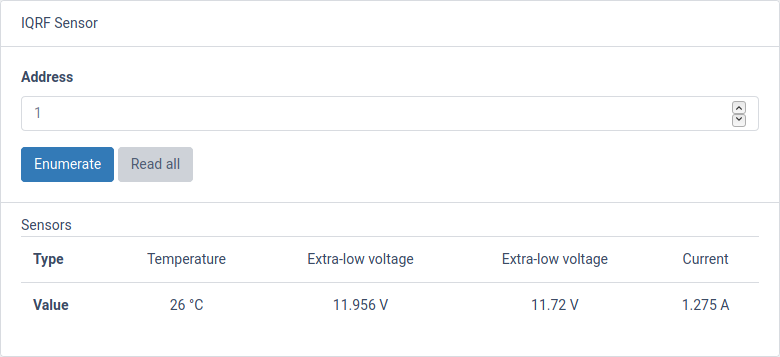
\includegraphics[width = 0.75\textwidth]{img/iqrf-gateway-webapp.png}
        \caption{Snímek obrazovky s vyčtenými hodnotami z aplikace IQRF Gateway Webapp}
      \end{figure}

	\section{Schéma zapojení}	
	
	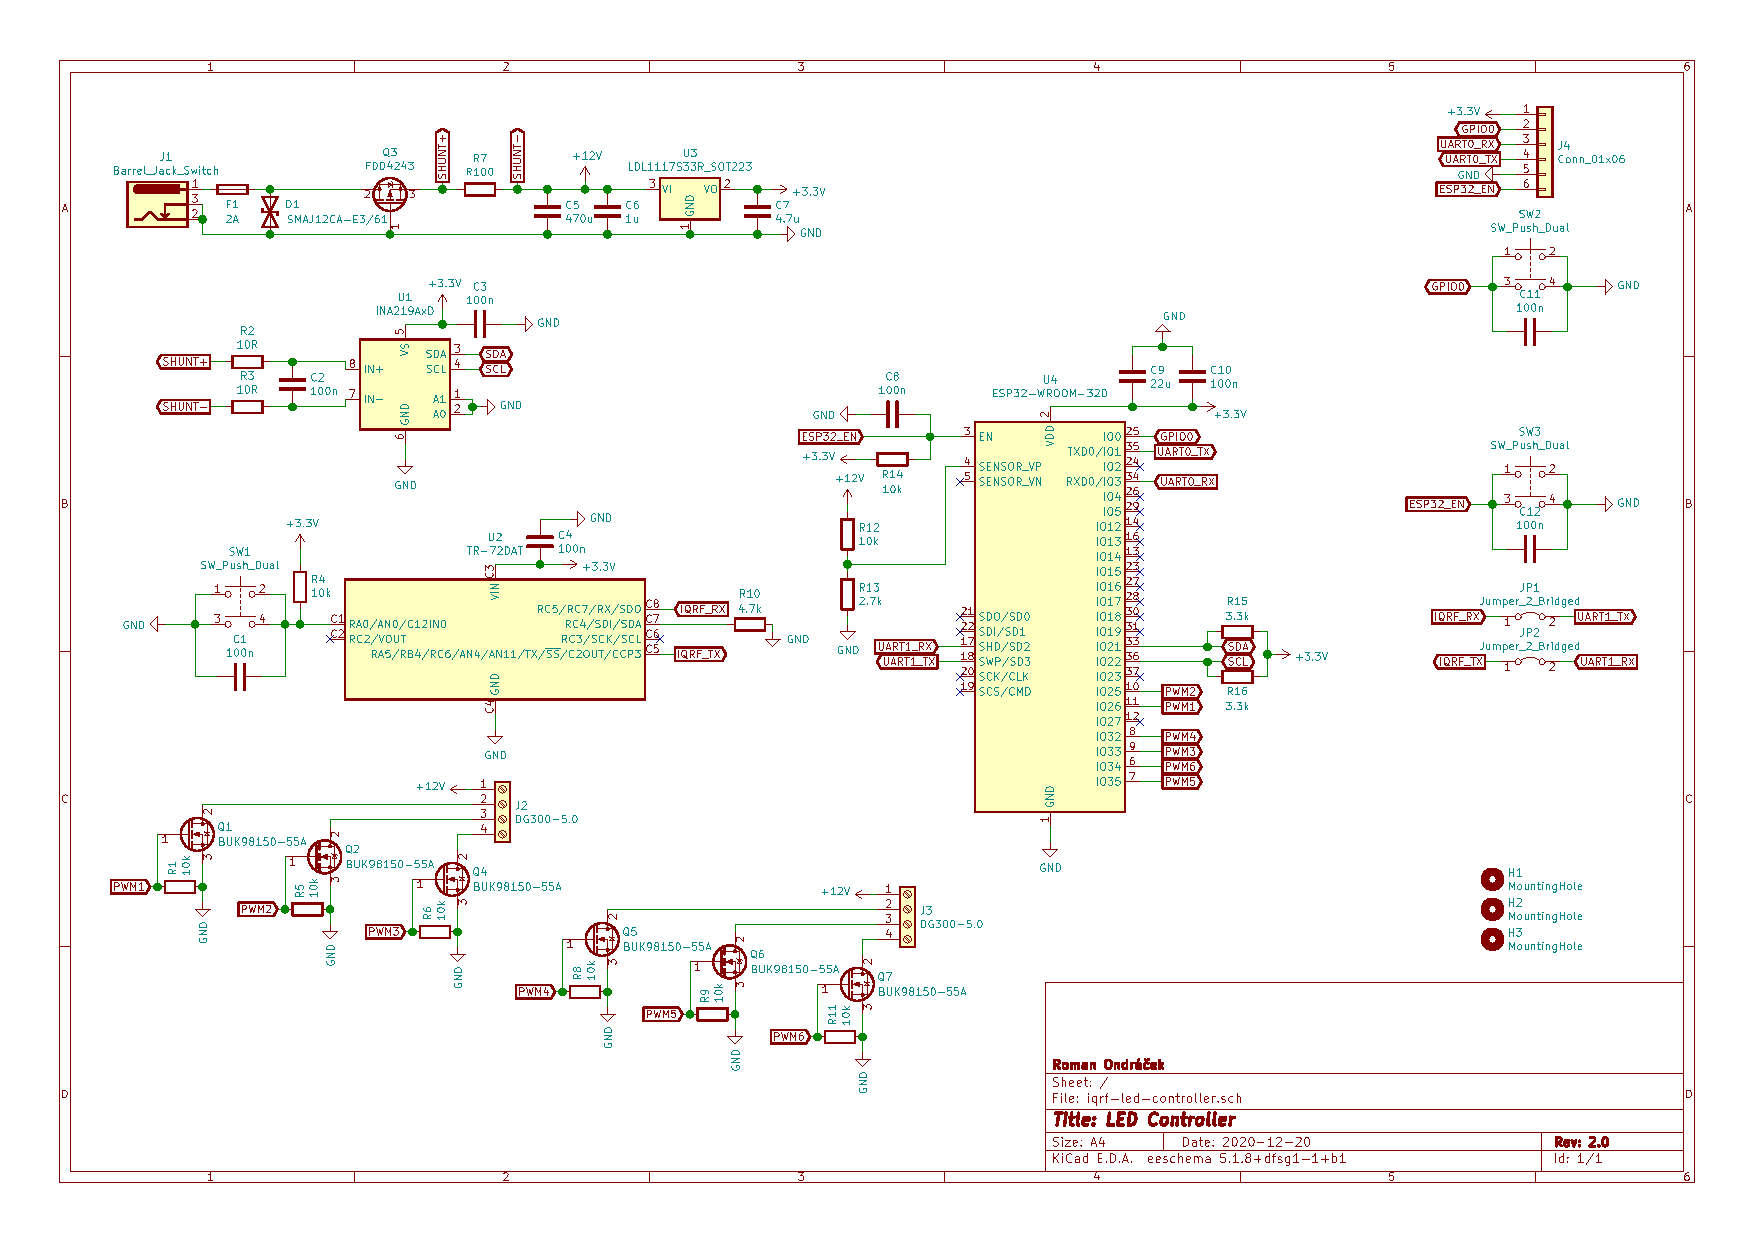
\includegraphics[scale=0.79,angle=90]{img/schema.pdf}	
	
	\section{Způsob řešení}	
	
	O veškerou logiku se stará ESP32, které komunikuje s IQRF modulem po rozhraní UART, pomocí ADC a odporového děliče měří vstupní napětí a pomocí PWM reguluje intenzitu osvětlení. Dále ESP32 se stará o komunikaci se senzorem INA219 po sběrnici I2C. Části programu pro ESP32 byly převzaty z dokumentace aplikačního rámce ESP-IDF\footnote{\url{https://docs.espressif.com/projects/esp-idf/en/latest/esp32/index.html}}. Části Custom DPA handleru byly převzaty z ukázek z IQRF Startup balíčku\footnote{\url{https://static.iqrf.org/IQRF_Startup_Package_OS404D_TR-7xD_200918.zip}}.
	
	\section{Závěr}
	
	Navržený systém řízení a měření LED pásků byl navržen a realizován ve formě funkčního vzorku. Chybí implementace IQRF standardu pro světla. Dále v návrhu desky plošných spojů je chyba, které znemožňuje použití 2. a 3. kanálu pro 2. RGB LED pásek.
	
	Video naleznete na \url{https://www.romanondracek.cz/imp-new.mp4}.	
	
      \begin{figure}[!ht]
      	\centering
        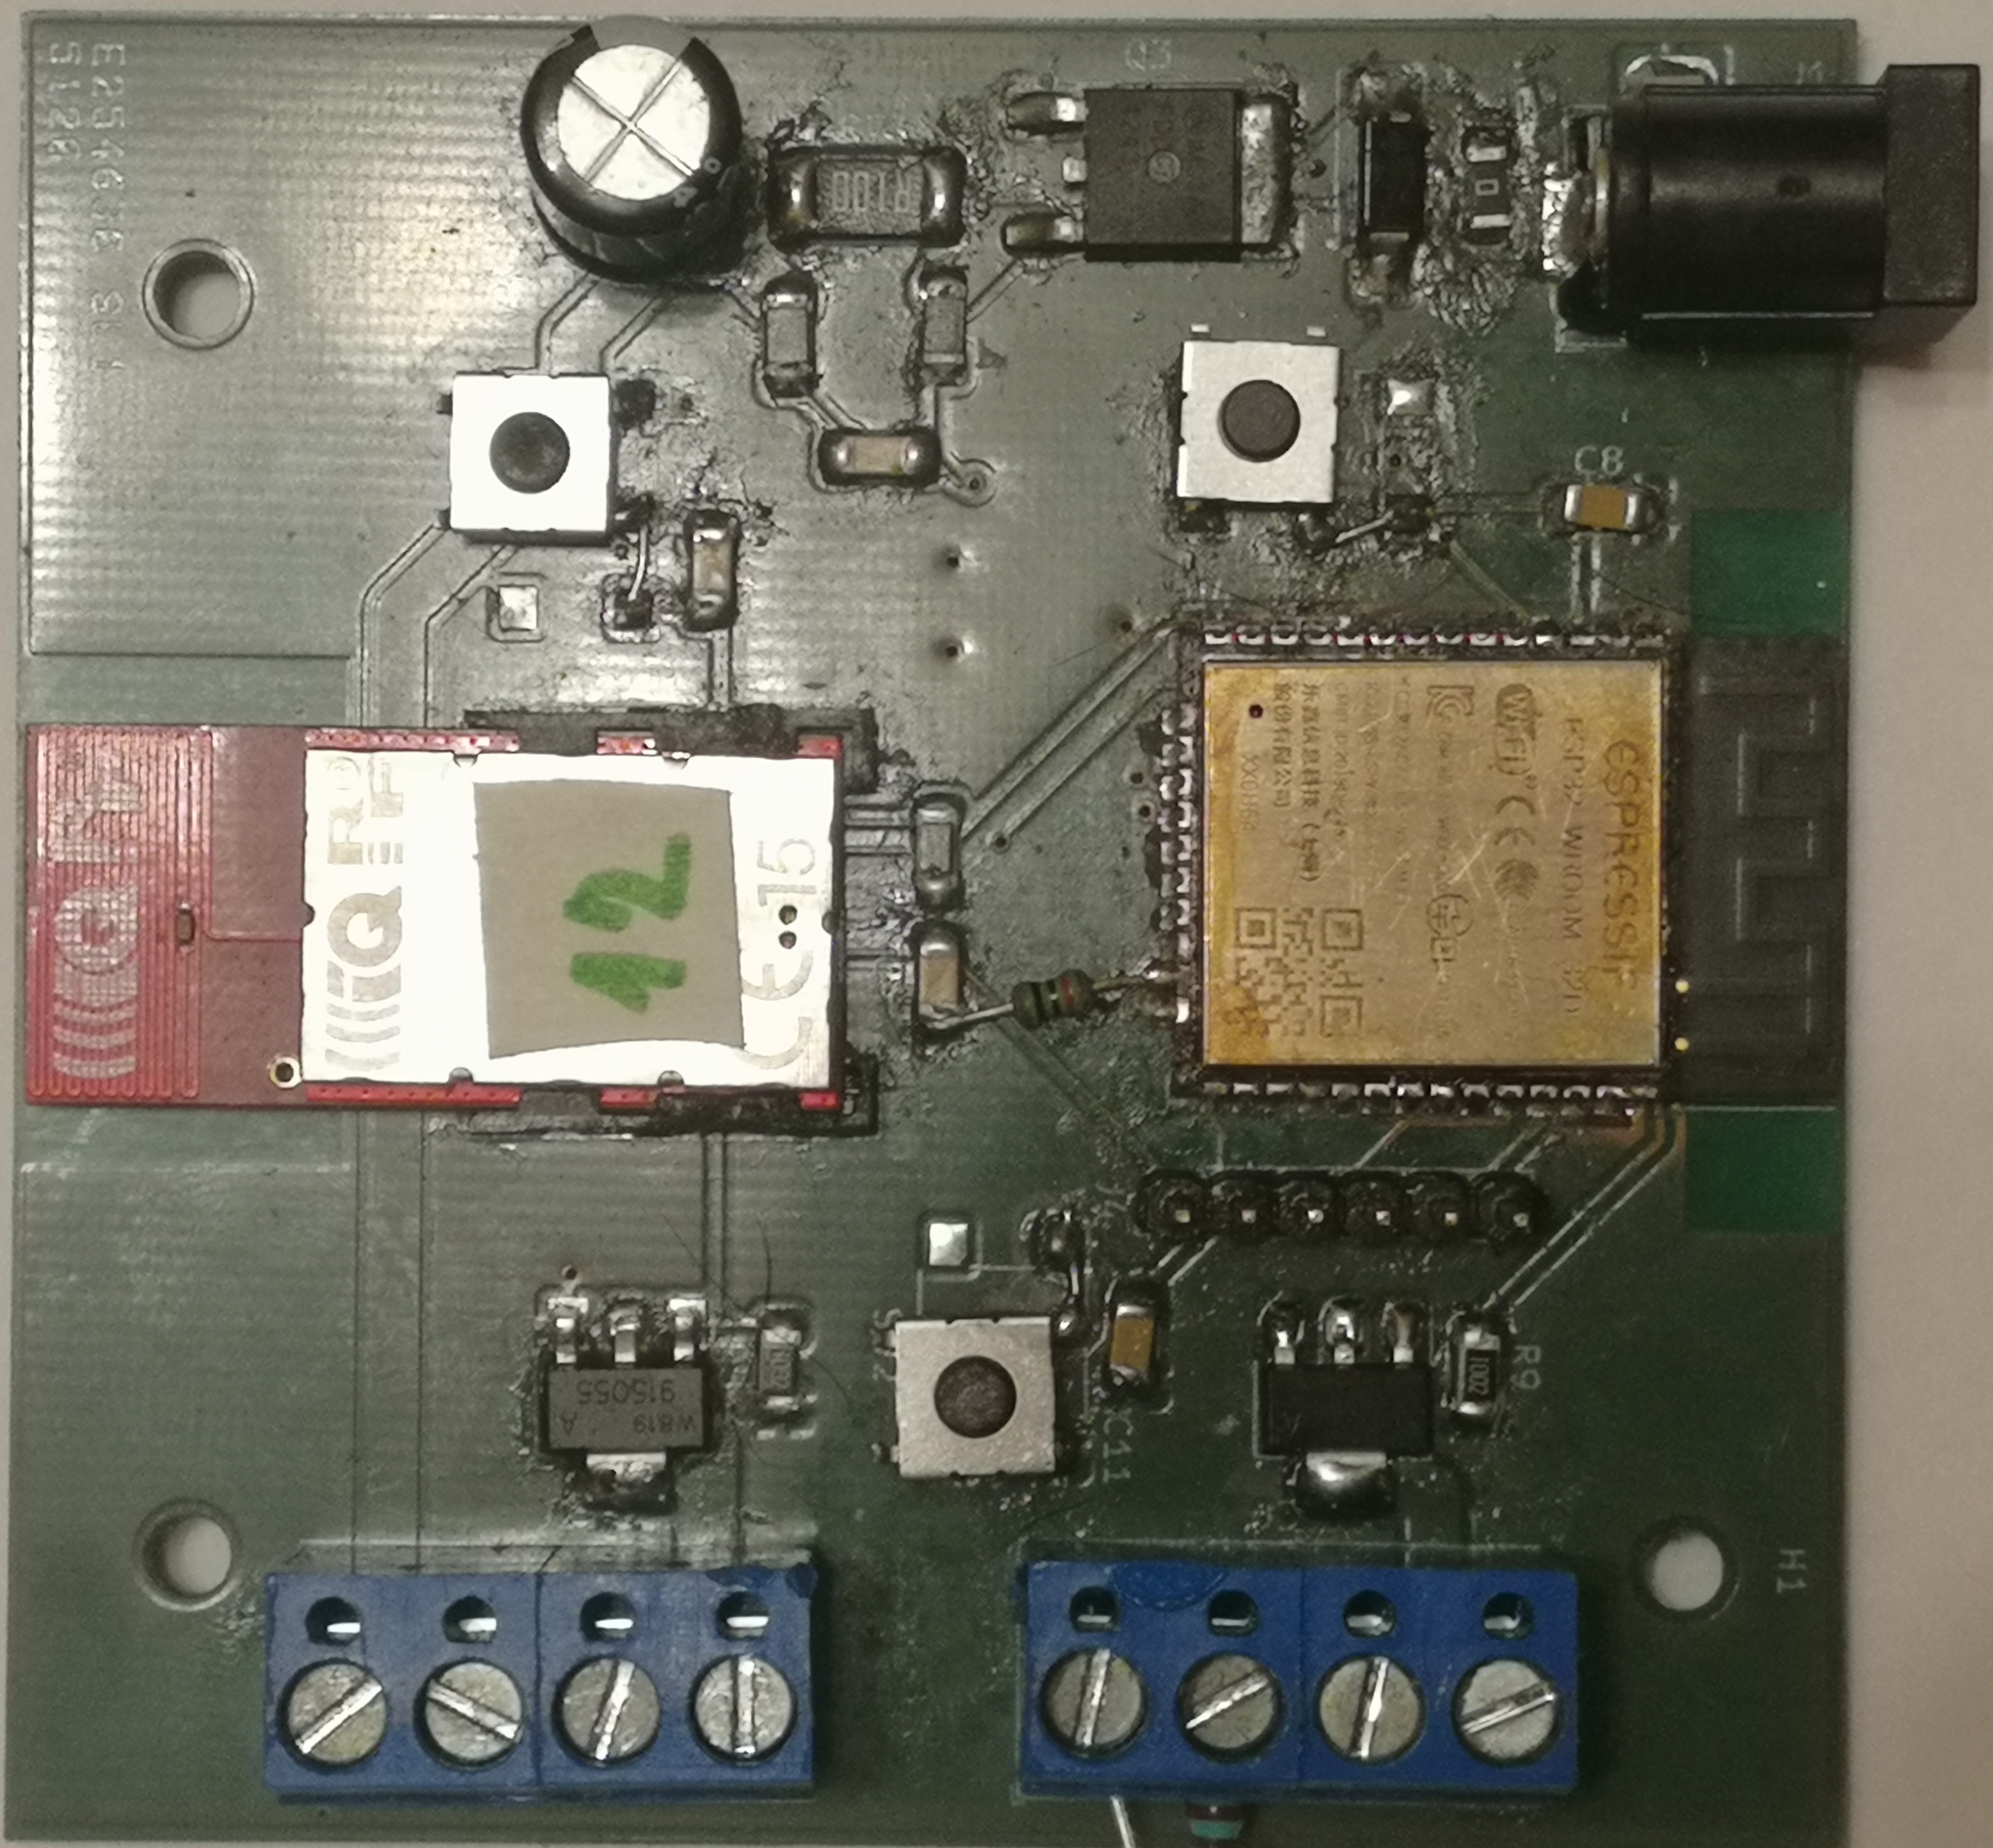
\includegraphics[width = 0.5\textwidth]{img/pcb-front.jpg}
        \caption{Fotografie LED Controlleru}
      \end{figure}	
      
      \begin{figure}[!ht]
      	\centering
        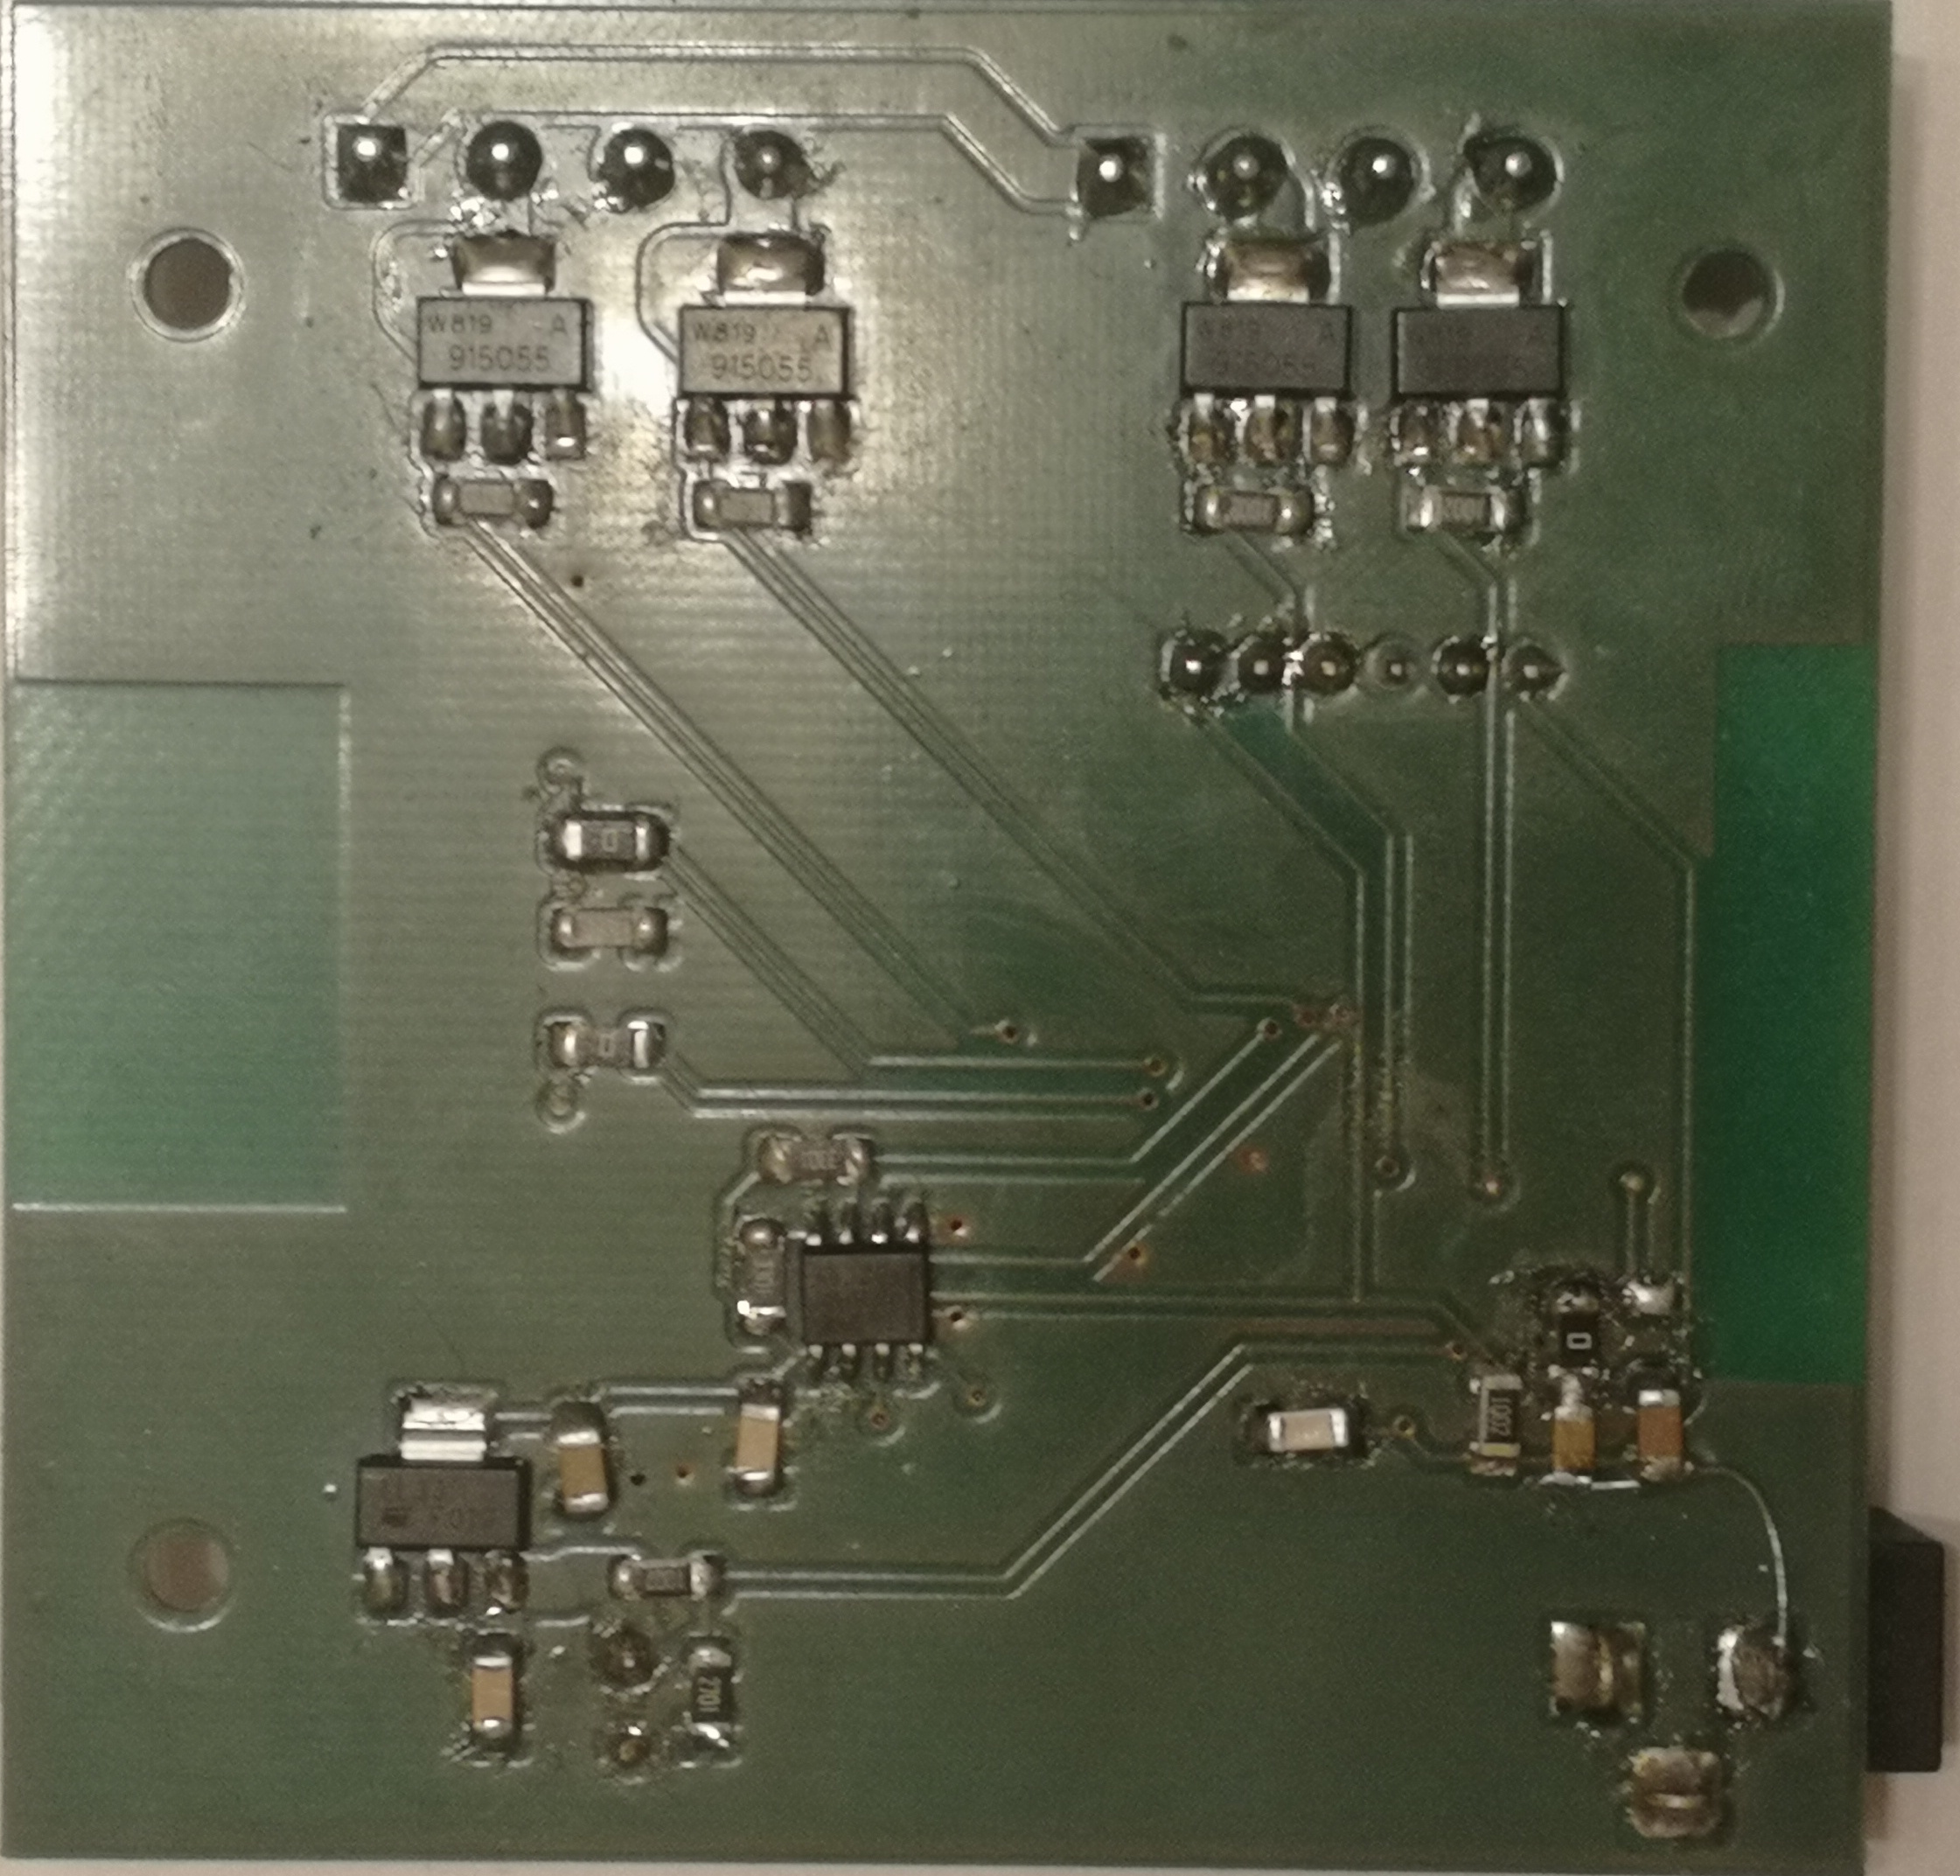
\includegraphics[width = 0.5\textwidth]{img/pcb-back.jpg}
        \caption{Fotografie LED Controlleru}
      \end{figure}
	
	\newpage
	
	\begin{thebibliography}{99}

\addcontentsline{toc}{section}{Seznam použité literatury}

\bibitem{led-controller}
ONDRÁČEK, Roman. LED Controller. \emph{LED Controller} [online]. Boskovice, 2016 [cit. 2020-12-24]. Dostupné z: \url{https://github.com/Roman3349/led-controller}

\bibitem{iqrf/ide}
IQRF Tech s.r.o. IQRF IDE \emph{IQRF} [online]. Jičín, 2020 [cit. 2020-12-24]. \\ Dostupné z: \url{https://www.iqrf.org/technology/iqrf-ide}

\bibitem{iqrf/os}
IQRF Tech s.r.o. Operating system \emph{IQRF} [online]. Jičín, 2020 [cit. 2020-12-24]. \\ Dostupné z: \url{https://www.iqrf.org/technology/operating-system}

\bibitem{iqrf/os/guide}
IQRF Tech s.r.o. IQRF OS v4.04D User's guide for TR-7xD \emph{IQRF} [online]. Jičín, 2020 [cit. 2020-12-24]. \\ Dostupné z: \url{https://static.iqrf.org/User_Guide_IQRF-OS-404D_TR-7xD_200918.pdf}

\bibitem{iqrf/dpa}
IQRF Tech s.r.o. DPA \emph{IQRF} [online]. Jičín, 2020 [cit. 2020-12-24]. \\ Dostupné z: \url{https://www.iqrf.org/technology/dpa}

\bibitem{iqrf/dpa/guide}
IQRF Tech s.r.o. DPA Framework Technical guide v4.15 \emph{IQRF} [online]. Jičín, 2020 [cit. 2020-12-24]. \\ Dostupné z: \url{https://static.iqrf.org/Tech_Guide_DPA-Framework-415_200903.pdf}

\bibitem{iqrf/dctr-72d-datasheet}
IQRF Tech s.r.o. Datasheet (DC)TR-72D \emph{IQRF} [online]. Jičín, 2020 [cit. 2020-12-24]. \\ Dostupné z: \url{https://static.iqrf.org/Datasheet_TR-72D_200525.pdf}

\bibitem{iqrf/standard-sensor}
IQRF Alliance IQRF Standard Sensor \emph{IQRF Alliance} [online]. Jičín, 2020 [cit. 2020-12-24]. \\ Dostupné z: \url{https://www.iqrfalliance.org/techdoc_files/IQRF-StandardSensor_V015.pdf}

\bibitem{iqrf/iqrf-gateway-daemon}
IQRF Tech s.r.o. IQRF Gateway Daemon \emph{IQRF} [online]. Jičín, 2020 [cit. 2020-12-24]. \\ Dostupné z: \url{https://gitlab.iqrf.org/open-source/iqrf-gateway-daemon}

\bibitem{iqrf/iqrf-gateway-webapp}
IQRF Tech s.r.o. IQRF Gateway Webapp \emph{IQRF} [online]. Jičín, 2020 [cit. 2020-12-24]. \\ Dostupné z: \url{https://gitlab.iqrf.org/open-source/iqrf-gateway-webapp}

\bibitem{microchip/pic16f1938}
Microchip. PIC16F1938 \emph{PIC16F1938} [online]. 2017 [cit. 2020-12-24]. \\ Dostupné z: \url{https://ww1.microchip.com/downloads/en/DeviceDoc/40001574D.pdf}

\bibitem{sw/kicad}
KiCad EDA \emph{KiCad EDA} [online]. 2020 [cit. 2020-12-24]. \\ Dostupné z: \url{http://kicad-pcb.org/}

\bibitem{sw/platformio-ide}
PlatormIO. PlatformIO IDE \emph{PlatformIO} [online]. 2020 [cit. 2020-12-24]. \\ Dostupné z: \url{https://platformio.org/platformio-ide}


\end{thebibliography}
\end{document}